\chapter{Case study}
This chapter presents a case study where the load forecasting system is applied to Bruny Island.
As discussed in section \ref{scope} (\nameref{scope}), the aim of this case study is to develop a load forecasting system which can predict future load based on weather, holiday periods, car movement, and other factors. 
Bruny Island and the NAC will be used as a case study. 
The forecasting system is expected to be equally applicable to any power system network, \hl{and this will be demonstrated later in this chapter}.
\\
Specifically, the system will have the following properties:
\begin{itemize}
	\item The system will produce a forecast up to 24 hours in the future in 15- to 60-minute intervals. This will be a rolling forecast that can be re-calculated at any time.
	\item The forecast will be able to begin from any point time.
	\item The forecast will predict load in kVA at each interval.
	\item The forecast system will be aimed at predicting aggregate load at the feeder level. That is, between approximately 0.5 and 10MVA.
	\item The forecast system will be especially tuned to predict load during holiday periods.
\end{itemize}

\begin{figure}
	\centering
	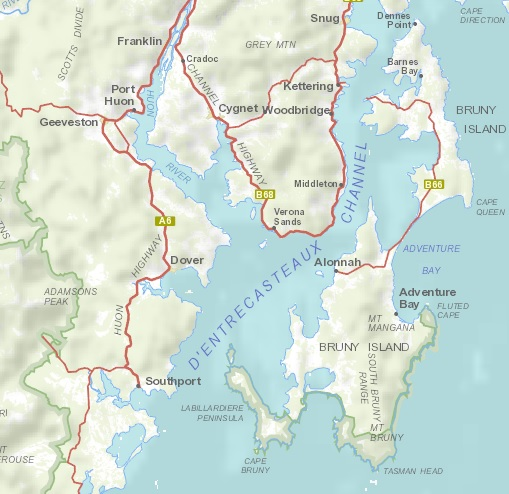
\includegraphics[width=0.35\linewidth]{images/bruny-basic}
	\caption{Bruny Island, in southern Tasmania, Australia. TODO: make a map that has expanded views to show the location on world map. QGIS, perhaps.}
	\label{fig:bruny-basic}
\end{figure}

\section{Bruny Island}
Bruny Island is located in south-east Tasmania, shown in figure \ref{fig:bruny-basic}.
The island has a population of around 620 people and is a popular destination in holiday periods, at which times the population swells considerably (\hl{reference the next section}).
\par
Power is supplied to the island via two submarine cables.
One cable supplies a small area in the North of the island, while the other supplies the remainder of the island to the South.
The two areas are connected by a recloser which is left in an open state during normal operation.
That is, the two areas on the island are not connected.
Additionally, there is a diesel generator in the southern section of the island which can be switched on by power system operators to reduce the load flowing through the submarine cable.
This is generally required during periods of peak demand, such as holidays.
This case study will look exclusively at the southern section of the island.
Figure (\hl{xx}) shows the layout of the power network on the island.
(\hl{Reclosers R1, R2, and R3 are located at Kettering, before Alonnah, and before Adventure Bay, respectively.})

There are no roads to Bruny Island - only a single ferry route.
It is also possible for people to arrive on the island by personal boat, but the number of people doing this is assumed to be negligible.
This single entry/exit point makes it possible to monitor the movement of traffic arriving on and departing the island, which will be investigated.



\section{Data analysis}
\label{bruny-data-analysis}
\hl{This section really rambles - it will be cut down a lot.}
\begin{itemize}
	\item \hl{this dot point list is for planning}
	\item discuss available data - load, weather, cars, other feeders and reclosers
	\item general load profiles of winter week, summer week, and full year
	\item look at annual growth of electricity. I need to investigate further my graph that is anomalous for 2013 and 2014 in growth.
	\item talk about different days of the week, and relate to car movement
	\item Look at special days - easter, june, christmas/ny
	\item talk about relationship between load and weather - temperature mainly
	\item Is load influenced by humidity like literature claims, or are temperature and humidity simply related?
	\item look at coloured scatter plot of load, temperature, and cumulative cars - more people correlates with more load in general - but we don't know future number of people.
	\item correlation matrix for power, cars, and weather
	\item cross correlations. Especially discuss any lags
	\item perhaps conclude with some important takeaways
	
\end{itemize}

In section \ref{patterns-profiles} the general properties of load profiles and how they are influenced by exogenous factors was discussed. Now, these general properties will be investigated in depth for the particular feeder in the case study.
\subsection{Available data}
The following data is available:
\todo[inline]{replace with a table}
\begin{itemize}
	\item kVA supplied through recloser R1 in 60 minute resolution between January 1, 2007 and March 9, 2012
	\item kVA supplied through recloser R1 in 5 minute resolution between March 9, 2012 and March 24, 2018
	\item kVA supplied to the feeder that R1 is connected to in 60 minute resolution between May 28, 2012 and March 24, 2018
	\item Ambient Temperature, solar irradiance, humidity, and wind speed at Lenah Valley between September 17, 2009 and March 24, 2018
	\item Vehicle movement data in 10 minute resolution between June 4, 2015 and March 24, 2018
\end{itemize}	
Vehicle movement data is provided as a set of observations every 10 minutes recording the number of vehicles arriving on the island, and the number of vehicles departing the island.
By integrating this, a relative number of vehicles on the island can be established.

There is a significant amount of bad or missing data throughout these datasets.
This has been handled by limiting the use of data where there are too many missing or bad values, as discussed later in this chapter.	


\subsection{Analysis}
Let's begin by having a simple look at some load profiles from the island.
Figure \ref{fig:load-profiles} shows apparent power draw on Bruny Island over a winter week, a summer week, and over an entire year.
These two weeks were selected to avoid special days such as holidays and are representative of typical weeks.
Some observations are immediately obvious
\begin{itemize}
	\item The midday load is only marginally larger than the overnight load in summer, but in winter it is significantly larger.
	\item Morning peaks are larger than afternoon peaks in summer, but in winter they are approximately equal.
	\item Thursday midday of the summer week appears abnormally high - perhaps this is a special day.
	\item There is some bad data on Tuesday of the summer week, as well as some missing data throughout the year.
	\item Over the whole year there appears to be a trend of increased max daily load over winter, which coincides with colder weather. This can be seen in the two individual weeks also.
	\item There are some periods of abnormally large load over the year: March 27, June 11, and December 28.
\end{itemize}

\begin{figure}[htbp]
	\centering
	\subfigure[]{
		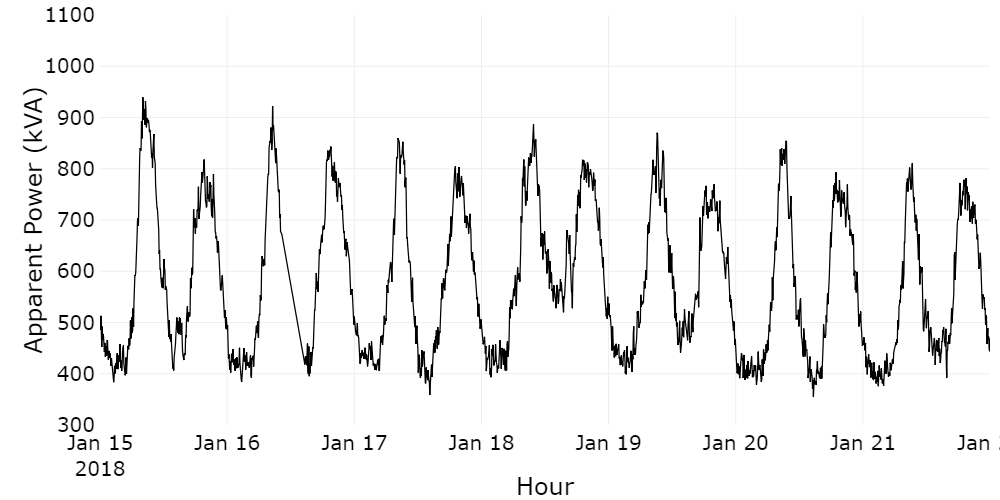
\includegraphics[width=0.8\textwidth]{images/simple-week-summer}
		\label{fig:simple-week-summer}}
	\vfil
	\subfigure[]{
		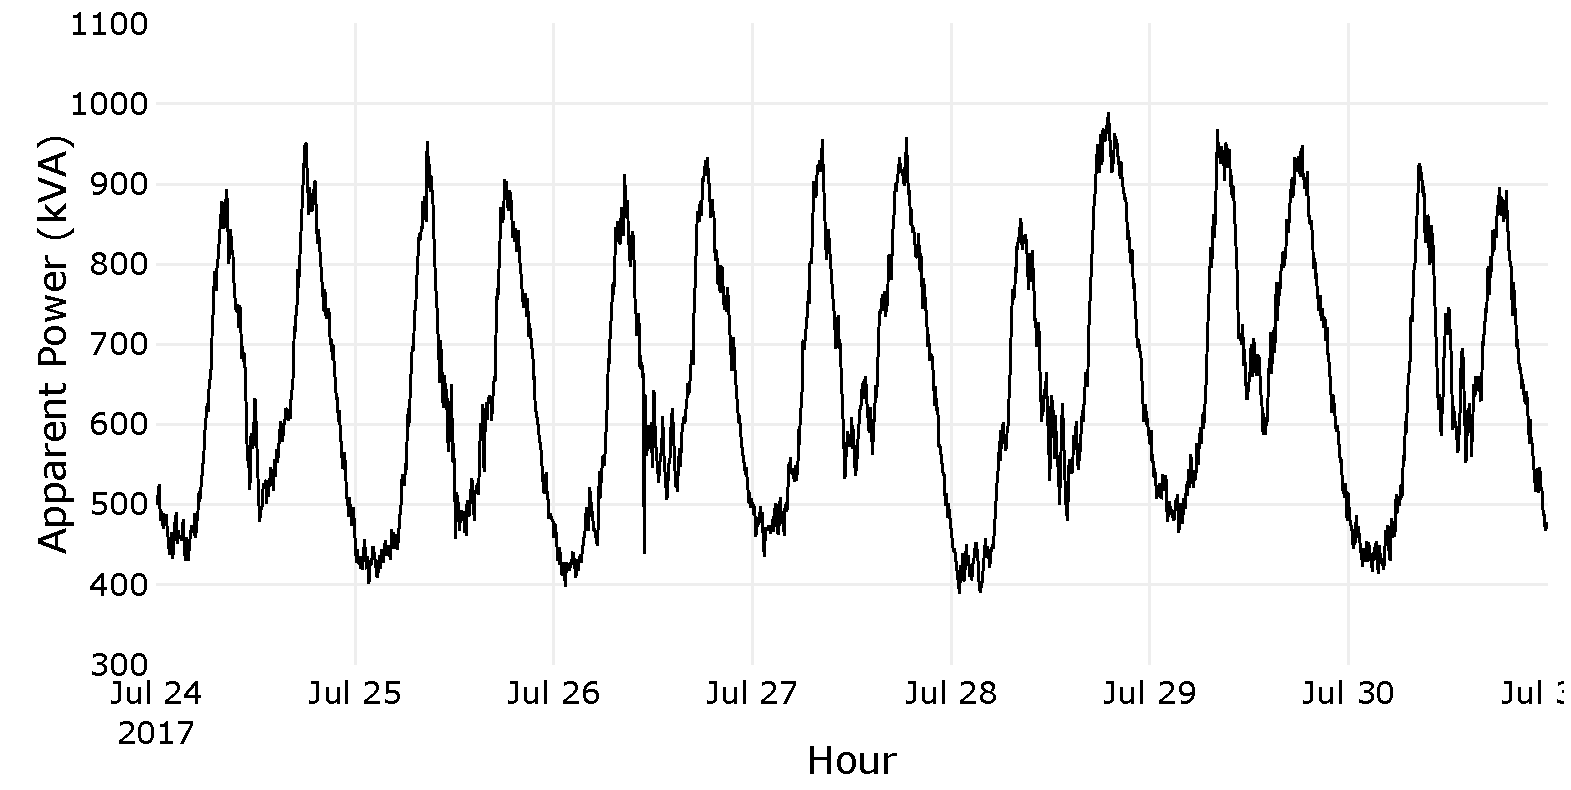
\includegraphics[width=0.8\textwidth]{images/simple-week-winter}
		\label{fig:simple-week-winter}}
	\vfil
	\subfigure[]{
		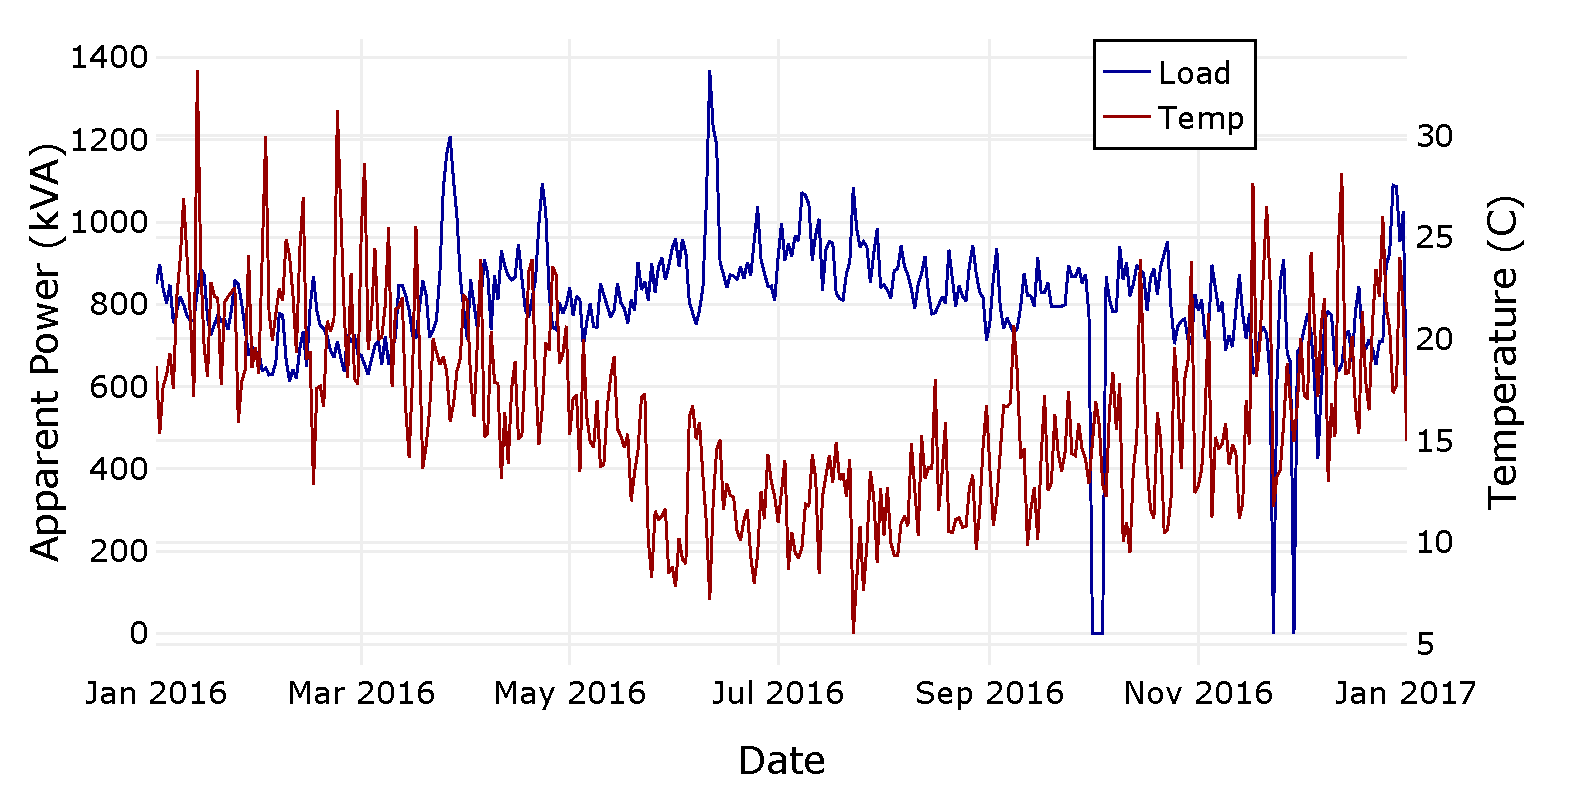
\includegraphics[width=0.8\textwidth]{images/max-load-max-temp}
		\label{fig:max-load-max-temp}}
	\caption{Bruny Island load profiles. (a) Load over a single summer week in 2018. (b) Load over a single winter week in 2017. (c) Peak daily load and peak daily temperature over all of 2017.}
	\label{fig:load-profiles}
\end{figure}

It was mentioned in section \ref{patterns-profiles} that weekends and weekdays tend to have different load profiles, but this is not immediately obvious from figure \ref{fig:load-profiles}.
Figure \ref{fig:average-profiles} shows this difference between days of the week.
What is immediately obviously is that the differences between days of the week are not restricted to 24 hour bounds - the different load profile shapes gently merge into each other over the course of an afternoon or morning.
% This is an especially important observation for a forecasting system that needs to be able to perform forecasts not just at a single time each day, but at any time.
It can be seen that the Friday profile morphs into the Saturday profile during the afternoon, perhaps as people arrive on the island for the weekend, and the Sunday profile morphs into a weekday profile over the afternoon, perhaps as people depart the island.
\par
Figures \ref{fig:average-arriving} and \ref{fig:average-departing} further support that the changes in load profiles are a result of people arriving on or leaving the island.
It can be seen that many vehicles tend to arrive on the island on Friday afternoon, leading to the change in load profile between Friday and Saturday.
Likewise, many vehicles leave the island on Sunday afternoon, shifting the load profile from Sunday to a weekday.

%This observation, that the load profiles on weekends and weekdays are only partially different, could indicate that information may be lost by considering only a single day.

\begin{figure}[htbp]
	\centering
	\subfigure[]{
		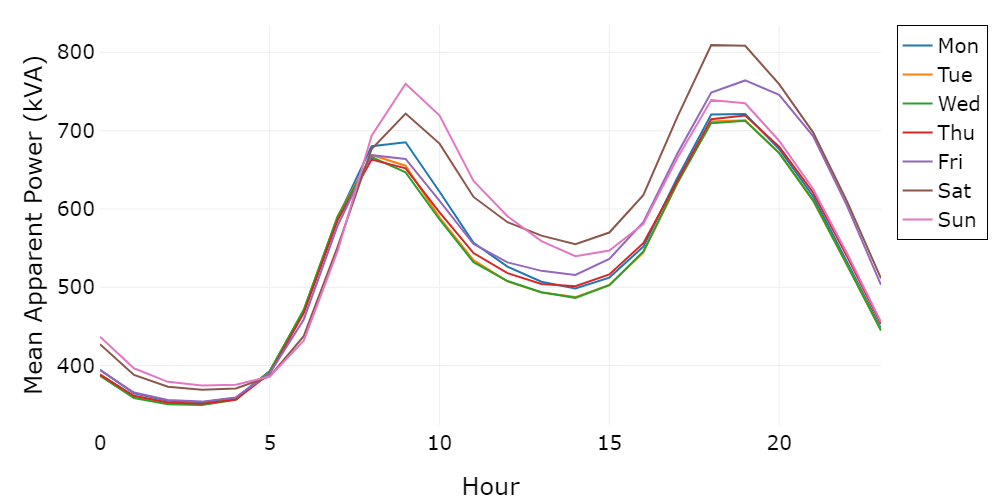
\includegraphics[width=.8\textwidth]{images/average-profiles}
		\label{fig:average-profiles}}
	\vfil
	\subfigure[]{
		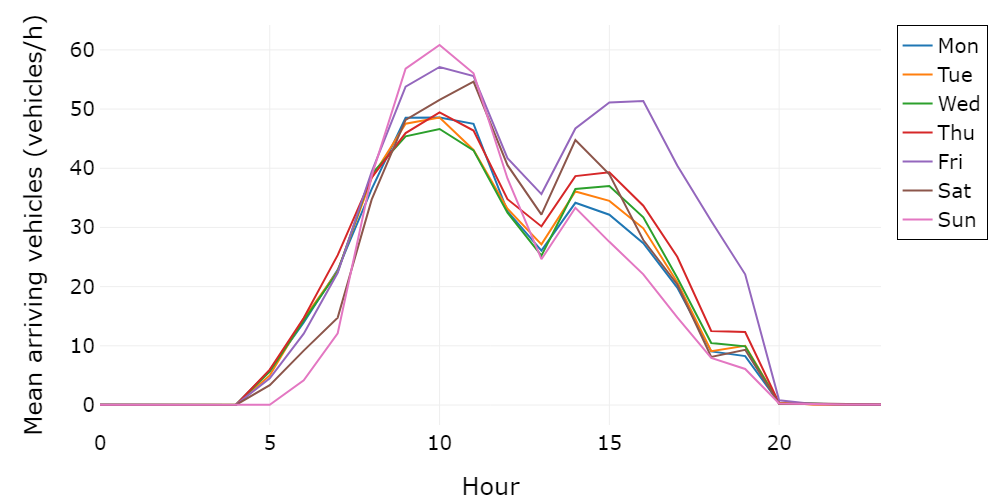
\includegraphics[width=.8\textwidth]{images/average-arriving}
		\label{fig:average-arriving}}
	\vfil
	\subfigure[]{
		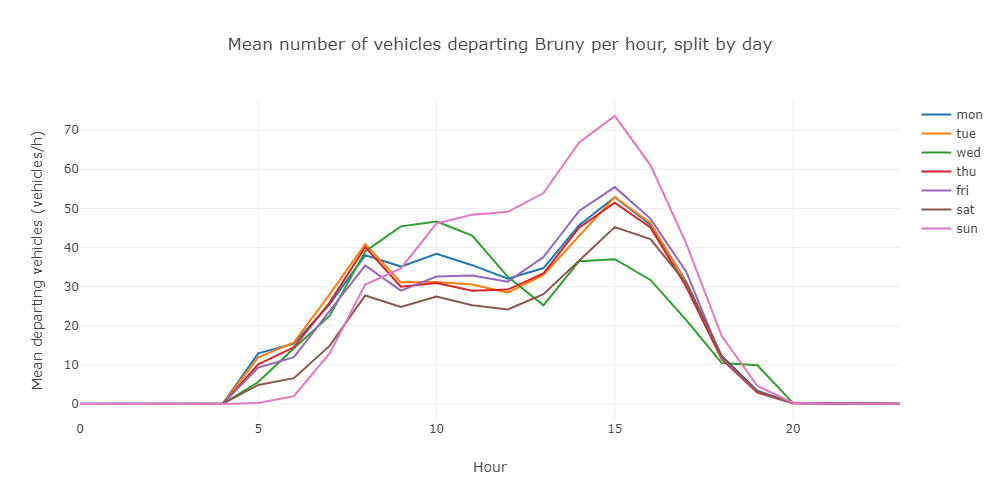
\includegraphics[width=.8\textwidth]{images/average-departing}
		\label{fig:average-departing}}
	\caption{Bruny Island average load profiles. (a) Average load profiles for each day of the week. Average number of cars arriving on (b) and leaving (c) the island each day.}
	\label{fig:average-load-profiles}
\end{figure}

Naturally, the next step is to attempt to look for clusters in the load profiles.
Looking at figure \ref{fig:all-monday-profiles}, there are no immediately obvious clusters.
However, it should be noted how the load profiles overnight have much lower variance than during the day - this will be important when evaluating the performance of the forecasting system if different models are used to forecast different hours of the day.

\begin{figure}
	\centering
	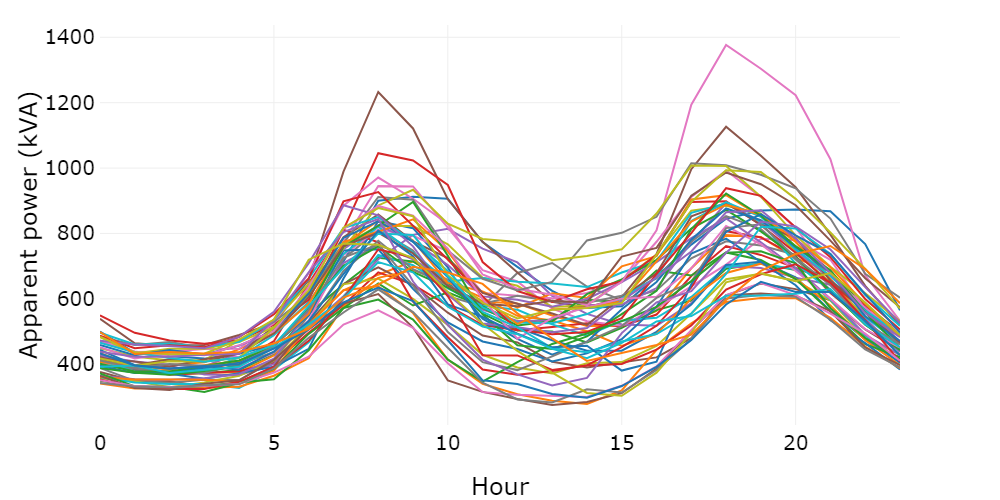
\includegraphics[width=0.8\linewidth]{images/all-monday-profiles}
	\caption{Load profiles of every Monday of 2017 overlaid. Notably, no clusters are immediately apparent in this plot.}
	\label{fig:all-monday-profiles}
\end{figure}


\section{Forecasting system architecture}
\begin{itemize}
	\item Transformer at core
	\item set of input vectors
	\item handling of bad data
	\item similar day selection
\end{itemize}


\section{Results}
\label{bruny-results}
Below are results from the current forecasting system.
The system takes the following data as input with 60 minute resolution:
\begin{itemize}
	\item Previous 24 hours of load
	\item Previous 24 through future 24 hours (total 48 hours) of temperature, humidity, holiday boolean flag, holiday ID (from 1 to $n$ depending on which holiday), day of week, and hour of day.
\end{itemize}

The system then produces the future 12 hours of load in 60 minute resolution.
The system is trained on data from October 1 2009 through October 1 2014, and is tested on data from October 2 2014 through April 30 2018.
All plots shown here are from the test dataset.


The below plots were specifically chosen to have an error that is close to the average, and to have the largest actual load. The intention is to give the best idea of how the system is currently performing on relatively difficult days.
It is expected that results will be considerably improved with the implementation of a similar day method.
\begin{figure}
	\centering
	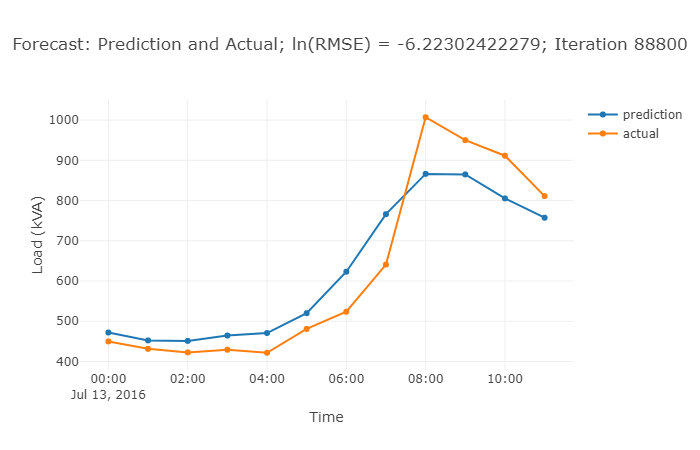
\includegraphics[width=0.95\linewidth]{images/prelim-plots/newplot}
	\caption{}
\end{figure}

\begin{figure}
\centering
\includegraphics[width=0.95\linewidth]{"images/prelim-plots/newplot (1)"}
\caption{}
\end{figure}

\begin{figure}
\centering
\includegraphics[width=0.95\linewidth]{"images/prelim-plots/newplot (2)"}
\caption{}
\end{figure}

\begin{figure}
\centering
\includegraphics[width=0.95\linewidth]{"images/prelim-plots/newplot (3)"}
\caption{}
\end{figure}

\begin{figure}
\centering
\includegraphics[width=0.95\linewidth]{"images/prelim-plots/newplot (4)"}
\caption{}
\end{figure}

\begin{figure}
\centering
\includegraphics[width=0.95\linewidth]{"images/prelim-plots/newplot (5)"}
\caption{}
\end{figure}

\begin{figure}
\centering
\includegraphics[width=0.95\linewidth]{"images/prelim-plots/newplot (6)"}
\caption{}
\end{figure}

\begin{figure}
\centering
\includegraphics[width=0.95\linewidth]{"images/prelim-plots/newplot (7)"}
\caption{}
\end{figure}

\begin{figure}
\centering
\includegraphics[width=0.95\linewidth]{"images/prelim-plots/newplot (8)"}
\caption{}
\end{figure}

\begin{figure}
\centering
\includegraphics[width=0.95\linewidth]{"images/prelim-plots/newplot (9)"}
\caption{}
\end{figure}

